% Options for packages loaded elsewhere
\PassOptionsToPackage{unicode}{hyperref}
\PassOptionsToPackage{hyphens}{url}
\PassOptionsToPackage{dvipsnames,svgnames,x11names}{xcolor}
%
\documentclass[
]{article}
\usepackage{amsmath,amssymb}
\usepackage{lmodern}
\usepackage{iftex}
\ifPDFTeX
  \usepackage[T1]{fontenc}
  \usepackage[utf8]{inputenc}
  \usepackage{textcomp} % provide euro and other symbols
\else % if luatex or xetex
  \usepackage{unicode-math}
  \defaultfontfeatures{Scale=MatchLowercase}
  \defaultfontfeatures[\rmfamily]{Ligatures=TeX,Scale=1}
\fi
% Use upquote if available, for straight quotes in verbatim environments
\IfFileExists{upquote.sty}{\usepackage{upquote}}{}
\IfFileExists{microtype.sty}{% use microtype if available
  \usepackage[]{microtype}
  \UseMicrotypeSet[protrusion]{basicmath} % disable protrusion for tt fonts
}{}
\makeatletter
\@ifundefined{KOMAClassName}{% if non-KOMA class
  \IfFileExists{parskip.sty}{%
    \usepackage{parskip}
  }{% else
    \setlength{\parindent}{0pt}
    \setlength{\parskip}{6pt plus 2pt minus 1pt}}
}{% if KOMA class
  \KOMAoptions{parskip=half}}
\makeatother
\usepackage{xcolor}
\IfFileExists{xurl.sty}{\usepackage{xurl}}{} % add URL line breaks if available
\IfFileExists{bookmark.sty}{\usepackage{bookmark}}{\usepackage{hyperref}}
\hypersetup{
  colorlinks=true,
  linkcolor={Maroon},
  filecolor={Maroon},
  citecolor={Blue},
  urlcolor={blue},
  pdfcreator={LaTeX via pandoc}}
\urlstyle{same} % disable monospaced font for URLs
\usepackage[margin=1in]{geometry}
\usepackage{color}
\usepackage{fancyvrb}
\newcommand{\VerbBar}{|}
\newcommand{\VERB}{\Verb[commandchars=\\\{\}]}
\DefineVerbatimEnvironment{Highlighting}{Verbatim}{commandchars=\\\{\}}
% Add ',fontsize=\small' for more characters per line
\usepackage{framed}
\definecolor{shadecolor}{RGB}{248,248,248}
\newenvironment{Shaded}{\begin{snugshade}}{\end{snugshade}}
\newcommand{\AlertTok}[1]{\textcolor[rgb]{0.94,0.16,0.16}{#1}}
\newcommand{\AnnotationTok}[1]{\textcolor[rgb]{0.56,0.35,0.01}{\textbf{\textit{#1}}}}
\newcommand{\AttributeTok}[1]{\textcolor[rgb]{0.77,0.63,0.00}{#1}}
\newcommand{\BaseNTok}[1]{\textcolor[rgb]{0.00,0.00,0.81}{#1}}
\newcommand{\BuiltInTok}[1]{#1}
\newcommand{\CharTok}[1]{\textcolor[rgb]{0.31,0.60,0.02}{#1}}
\newcommand{\CommentTok}[1]{\textcolor[rgb]{0.56,0.35,0.01}{\textit{#1}}}
\newcommand{\CommentVarTok}[1]{\textcolor[rgb]{0.56,0.35,0.01}{\textbf{\textit{#1}}}}
\newcommand{\ConstantTok}[1]{\textcolor[rgb]{0.00,0.00,0.00}{#1}}
\newcommand{\ControlFlowTok}[1]{\textcolor[rgb]{0.13,0.29,0.53}{\textbf{#1}}}
\newcommand{\DataTypeTok}[1]{\textcolor[rgb]{0.13,0.29,0.53}{#1}}
\newcommand{\DecValTok}[1]{\textcolor[rgb]{0.00,0.00,0.81}{#1}}
\newcommand{\DocumentationTok}[1]{\textcolor[rgb]{0.56,0.35,0.01}{\textbf{\textit{#1}}}}
\newcommand{\ErrorTok}[1]{\textcolor[rgb]{0.64,0.00,0.00}{\textbf{#1}}}
\newcommand{\ExtensionTok}[1]{#1}
\newcommand{\FloatTok}[1]{\textcolor[rgb]{0.00,0.00,0.81}{#1}}
\newcommand{\FunctionTok}[1]{\textcolor[rgb]{0.00,0.00,0.00}{#1}}
\newcommand{\ImportTok}[1]{#1}
\newcommand{\InformationTok}[1]{\textcolor[rgb]{0.56,0.35,0.01}{\textbf{\textit{#1}}}}
\newcommand{\KeywordTok}[1]{\textcolor[rgb]{0.13,0.29,0.53}{\textbf{#1}}}
\newcommand{\NormalTok}[1]{#1}
\newcommand{\OperatorTok}[1]{\textcolor[rgb]{0.81,0.36,0.00}{\textbf{#1}}}
\newcommand{\OtherTok}[1]{\textcolor[rgb]{0.56,0.35,0.01}{#1}}
\newcommand{\PreprocessorTok}[1]{\textcolor[rgb]{0.56,0.35,0.01}{\textit{#1}}}
\newcommand{\RegionMarkerTok}[1]{#1}
\newcommand{\SpecialCharTok}[1]{\textcolor[rgb]{0.00,0.00,0.00}{#1}}
\newcommand{\SpecialStringTok}[1]{\textcolor[rgb]{0.31,0.60,0.02}{#1}}
\newcommand{\StringTok}[1]{\textcolor[rgb]{0.31,0.60,0.02}{#1}}
\newcommand{\VariableTok}[1]{\textcolor[rgb]{0.00,0.00,0.00}{#1}}
\newcommand{\VerbatimStringTok}[1]{\textcolor[rgb]{0.31,0.60,0.02}{#1}}
\newcommand{\WarningTok}[1]{\textcolor[rgb]{0.56,0.35,0.01}{\textbf{\textit{#1}}}}
\usepackage{graphicx}
\makeatletter
\def\maxwidth{\ifdim\Gin@nat@width>\linewidth\linewidth\else\Gin@nat@width\fi}
\def\maxheight{\ifdim\Gin@nat@height>\textheight\textheight\else\Gin@nat@height\fi}
\makeatother
% Scale images if necessary, so that they will not overflow the page
% margins by default, and it is still possible to overwrite the defaults
% using explicit options in \includegraphics[width, height, ...]{}
\setkeys{Gin}{width=\maxwidth,height=\maxheight,keepaspectratio}
% Set default figure placement to htbp
\makeatletter
\def\fps@figure{htbp}
\makeatother
\setlength{\emergencystretch}{3em} % prevent overfull lines
\providecommand{\tightlist}{%
  \setlength{\itemsep}{0pt}\setlength{\parskip}{0pt}}
\setcounter{secnumdepth}{-\maxdimen} % remove section numbering
\ifLuaTeX
  \usepackage{selnolig}  % disable illegal ligatures
\fi

\title{Coupon Collector's Problem With Unequal Probabilities\\
\textbf{Application to Ecology}}
\author{Marko KACHAIKIN, Vincent RUNGE\\

\includegraphics[width=1in,height=\textheight]{logo_lamme.png}

\includegraphics[width=1.7in,height=\textheight]{logo_UEVE.png}}
\date{05/07/2022}

\begin{document}
\maketitle

{
\hypersetup{linkcolor=}
\setcounter{tocdepth}{2}
\tableofcontents
}
\noindent\hrulefill

\hypertarget{introduction}{%
\section{Introduction}\label{introduction}}

In this work we study the coupon collector's problem in the more generic
case of unequal occurrence probabilities. Our first goal consists in
better analyzing the probability distribution (mean and variance) for
the random variable of the time to completion for some particular cases.
We found simple formulas in asymptotic regime and compare these results
throughout an extensive simulation study.

Our secondary goal is the search for estimators for unknown coupon
number when we stop the collection at some chosen step. Performances of
proposed estimators are studied both theoretically and by simulations.

\begin{Shaded}
\begin{Highlighting}[]
\FunctionTok{library}\NormalTok{(coupon)}
\end{Highlighting}
\end{Shaded}

\hypertarget{from-equal-to-linear-probability-models}{%
\section{From equal to linear probability
models}\label{from-equal-to-linear-probability-models}}

We consider that the collection is made of \(N\) coupons with three
possibles models.

\begin{enumerate}
\def\labelenumi{\arabic{enumi}.}
\tightlist
\item
  the equal probability model:
\end{enumerate}

\[p_i = \frac{1}{N}\,,\quad i = 1,\ldots, N\,.\]

\begin{enumerate}
\def\labelenumi{\arabic{enumi}.}
\setcounter{enumi}{1}
\tightlist
\item
  the linear probability model:
\end{enumerate}

\[p_i = \frac{1}{N}\,,\quad i = 1,\ldots, N\,,\] with
\(\beta \in [0, \frac{2}{N(N-1)}]\).

\begin{enumerate}
\def\labelenumi{\arabic{enumi}.}
\setcounter{enumi}{2}
\tightlist
\item
  the 2-probability model:
\end{enumerate}

\[p_i = \frac{1}{N}\,,\quad i = 1,\ldots, N\,.\]

\hypertarget{the-log-linear-expectation-in-equality-case}{%
\subsection{The log-linear expectation in equality
case}\label{the-log-linear-expectation-in-equality-case}}

In case 1 we can easily verify the well-known asymptotic result:

\[\mathbb E [T] \approx N(\ln N + \gamma)\]

For \(N \in \{1,...,200\}\) we simulate \(10^3\) coupon problems. We
show the detailed code using our package \texttt{coupon} available on
GitHub (\url{https://github.com/vrunge/coupon})

\begin{Shaded}
\begin{Highlighting}[]
\NormalTok{res\_coupon }\OtherTok{\textless{}{-}} \ControlFlowTok{function}\NormalTok{(n, }\AttributeTok{nb\_iterations =} \DecValTok{10}\NormalTok{)}
\NormalTok{\{}
  \FunctionTok{mean}\NormalTok{(}\FunctionTok{replicate}\NormalTok{(nb\_iterations, }\FunctionTok{simu.coupon}\NormalTok{(}\AttributeTok{nbCoupons =}\NormalTok{ n)))}
\NormalTok{\}}
\NormalTok{res\_theory }\OtherTok{\textless{}{-}} \ControlFlowTok{function}\NormalTok{(n)\{n}\SpecialCharTok{*}\NormalTok{(}\FunctionTok{log}\NormalTok{(n) }\SpecialCharTok{{-}} \FunctionTok{digamma}\NormalTok{(}\DecValTok{1}\NormalTok{))\}}

\NormalTok{N }\OtherTok{\textless{}{-}} \DecValTok{200}
\NormalTok{moyenne\_resultat1 }\OtherTok{\textless{}{-}} \FunctionTok{sapply}\NormalTok{(}\DecValTok{1}\SpecialCharTok{:}\NormalTok{N, res\_coupon)}
\NormalTok{moyenne\_theorique }\OtherTok{\textless{}{-}} \FunctionTok{sapply}\NormalTok{(}\DecValTok{1}\SpecialCharTok{:}\NormalTok{N, res\_theory)}
\FunctionTok{plot}\NormalTok{(moyenne\_resultat1, }\AttributeTok{xlab =} \StringTok{"Nombre de coupons"}\NormalTok{, }\AttributeTok{ylab =} \StringTok{"Nombre d\textquotesingle{}articles à acheter"}\NormalTok{)}
\FunctionTok{lines}\NormalTok{(moyenne\_theorique)}
\end{Highlighting}
\end{Shaded}

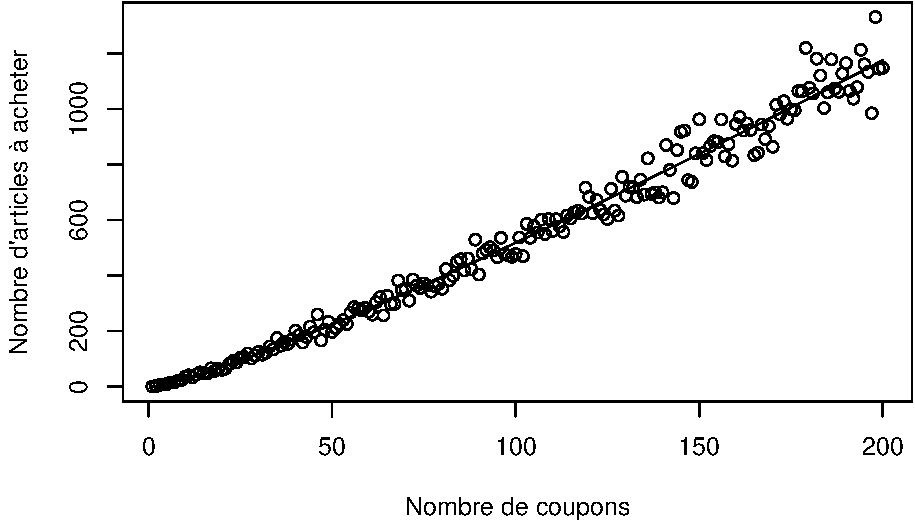
\includegraphics{examples_files/figure-latex/unnamed-chunk-2-1.pdf}

\hypertarget{estimation-of-n}{%
\section{Estimation of N}\label{estimation-of-n}}

\hypertarget{a-nice-picture}{%
\subsection{A nice picture}\label{a-nice-picture}}

We give a few examples of dynamics in the coupon problem. The x-axis
represents the time dynamics and the colors the number of observations
for each coupon sorted from the highest occcurrence (bottom) to the
smallest (0 if collection not completed) (top)

\begin{Shaded}
\begin{Highlighting}[]
\NormalTok{nbCoupons }\OtherTok{\textless{}{-}} \DecValTok{200}
\NormalTok{myN }\OtherTok{\textless{}{-}} \DecValTok{1000}
\FunctionTok{image}\NormalTok{(res }\OtherTok{\textless{}{-}} \FunctionTok{dynamicCollection}\NormalTok{(}\AttributeTok{nbCoupons =}\NormalTok{ nbCoupons, }\AttributeTok{N =}\NormalTok{ myN))}
\end{Highlighting}
\end{Shaded}

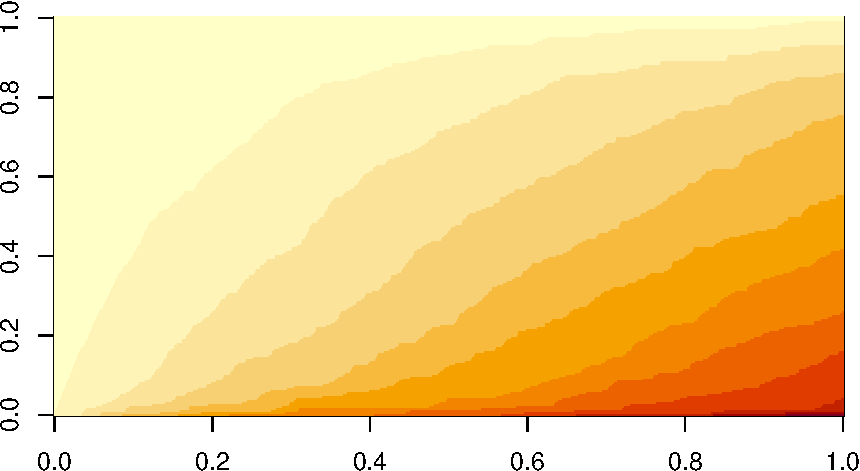
\includegraphics{examples_files/figure-latex/unnamed-chunk-3-1.pdf}

\begin{Shaded}
\begin{Highlighting}[]
\FunctionTok{image}\NormalTok{(res}\SpecialCharTok{\textgreater{}}\DecValTok{0}\NormalTok{)}
\end{Highlighting}
\end{Shaded}

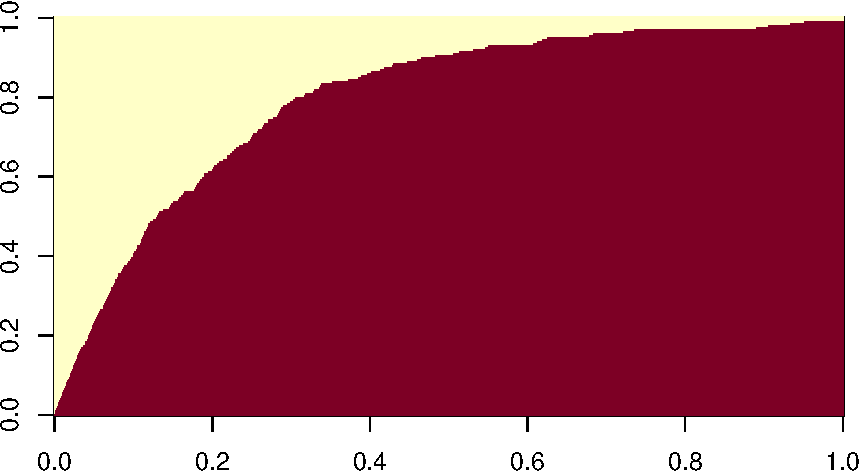
\includegraphics{examples_files/figure-latex/unnamed-chunk-3-2.pdf}

\begin{Shaded}
\begin{Highlighting}[]
\FunctionTok{image}\NormalTok{(res}\SpecialCharTok{==}\DecValTok{1}\NormalTok{)}
\end{Highlighting}
\end{Shaded}

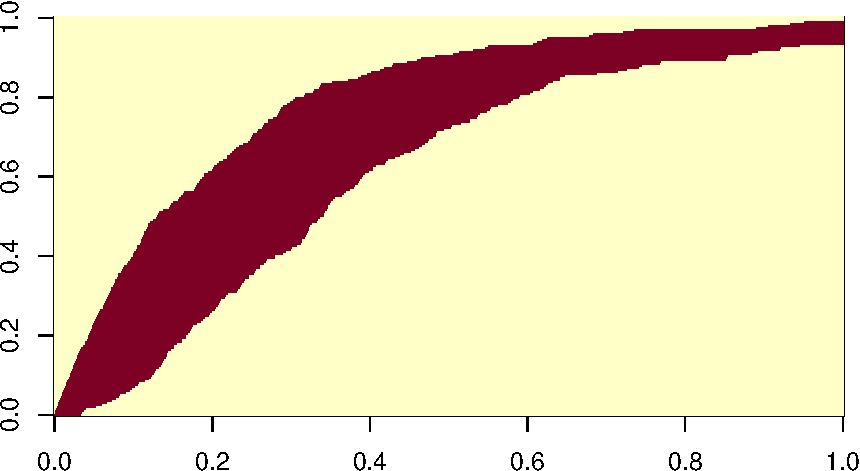
\includegraphics{examples_files/figure-latex/unnamed-chunk-3-3.pdf}

\begin{Shaded}
\begin{Highlighting}[]
\NormalTok{nbCoupons }\OtherTok{\textless{}{-}} \DecValTok{500}
\NormalTok{myN }\OtherTok{\textless{}{-}} \DecValTok{1000}
\FunctionTok{image}\NormalTok{(res }\OtherTok{\textless{}{-}} \FunctionTok{dynamicCollection}\NormalTok{(}\AttributeTok{nbCoupons =}\NormalTok{ nbCoupons, }\AttributeTok{N =}\NormalTok{ myN))}
\end{Highlighting}
\end{Shaded}

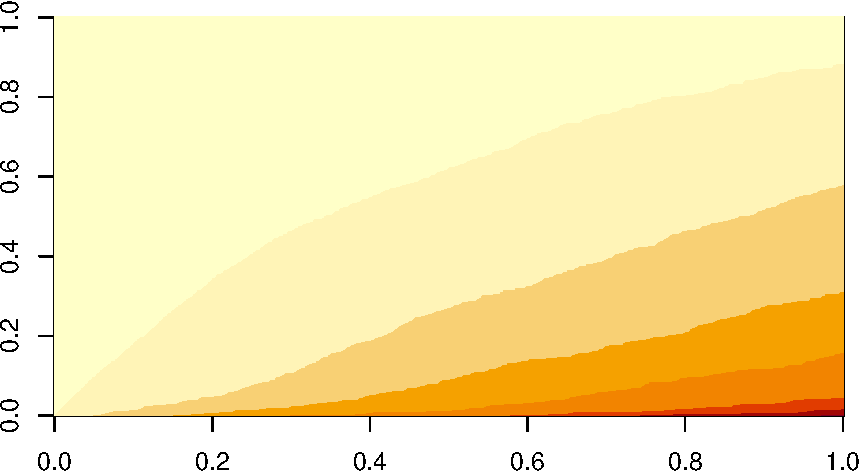
\includegraphics{examples_files/figure-latex/unnamed-chunk-4-1.pdf}

\begin{Shaded}
\begin{Highlighting}[]
\FunctionTok{image}\NormalTok{(res}\SpecialCharTok{\textgreater{}}\DecValTok{0}\NormalTok{)}
\end{Highlighting}
\end{Shaded}

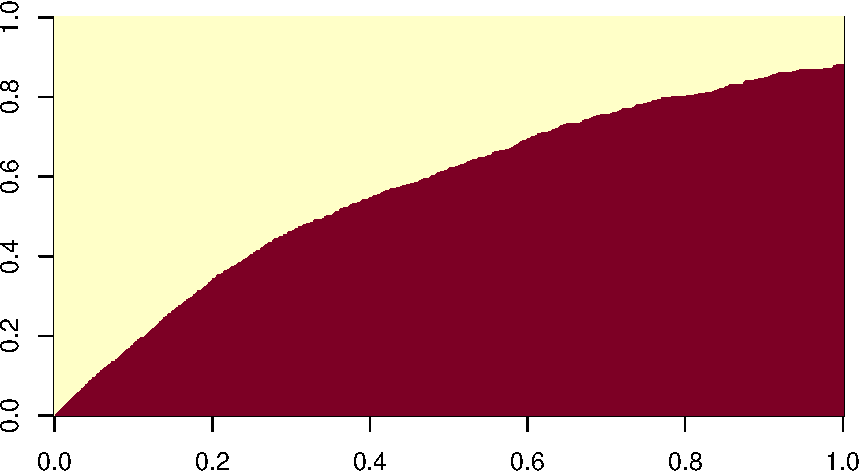
\includegraphics{examples_files/figure-latex/unnamed-chunk-4-2.pdf}

\begin{Shaded}
\begin{Highlighting}[]
\FunctionTok{image}\NormalTok{(res}\SpecialCharTok{==}\DecValTok{1}\NormalTok{)}
\end{Highlighting}
\end{Shaded}

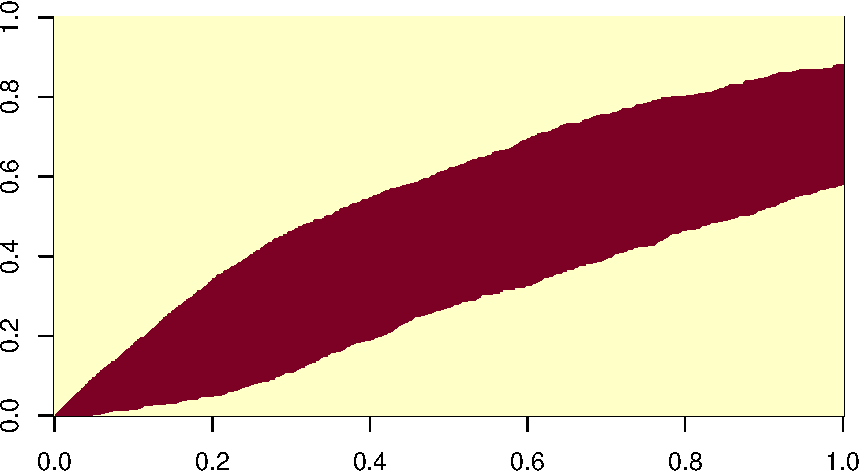
\includegraphics{examples_files/figure-latex/unnamed-chunk-4-3.pdf}

\begin{Shaded}
\begin{Highlighting}[]
\NormalTok{nbCoupons }\OtherTok{\textless{}{-}} \DecValTok{1000}
\NormalTok{myN }\OtherTok{\textless{}{-}} \DecValTok{1000}
\FunctionTok{image}\NormalTok{(res }\OtherTok{\textless{}{-}} \FunctionTok{dynamicCollection}\NormalTok{(}\AttributeTok{nbCoupons =}\NormalTok{ nbCoupons, }\AttributeTok{N =}\NormalTok{ myN))}
\end{Highlighting}
\end{Shaded}

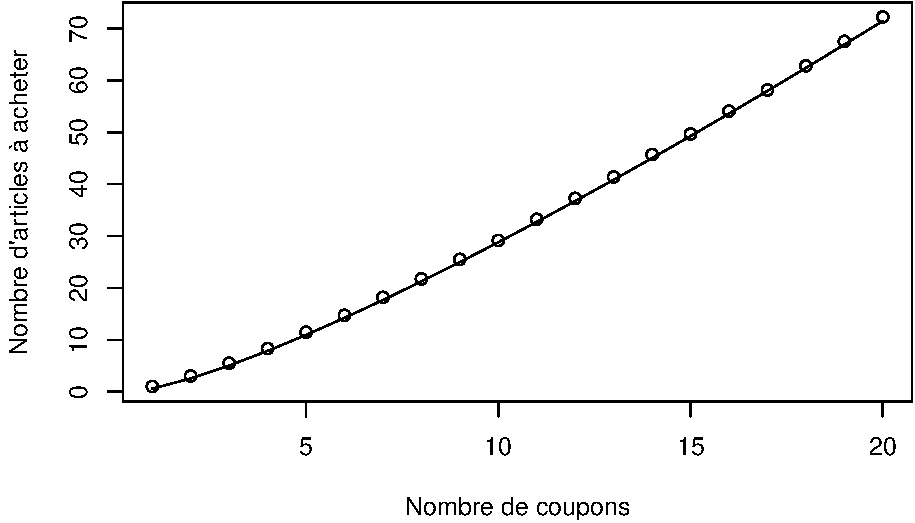
\includegraphics{examples_files/figure-latex/unnamed-chunk-5-1.pdf}

\begin{Shaded}
\begin{Highlighting}[]
\FunctionTok{image}\NormalTok{(res}\SpecialCharTok{\textgreater{}}\DecValTok{0}\NormalTok{)}
\end{Highlighting}
\end{Shaded}

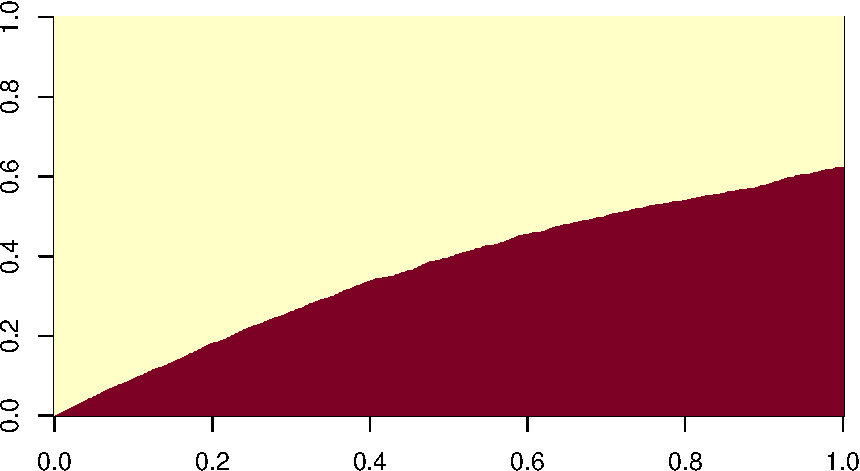
\includegraphics{examples_files/figure-latex/unnamed-chunk-5-2.pdf}

\begin{Shaded}
\begin{Highlighting}[]
\FunctionTok{image}\NormalTok{(res}\SpecialCharTok{==}\DecValTok{1}\NormalTok{)}
\end{Highlighting}
\end{Shaded}

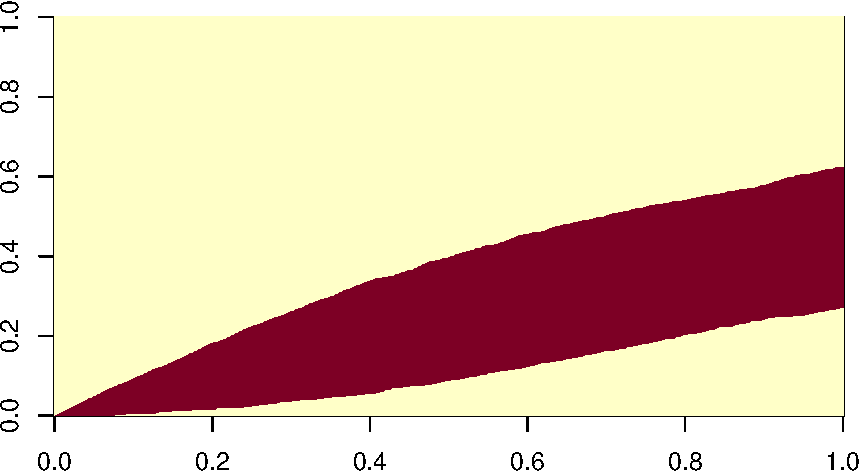
\includegraphics{examples_files/figure-latex/unnamed-chunk-5-3.pdf}

\hypertarget{moment-estimation}{%
\subsection{Moment estimation}\label{moment-estimation}}

The expected number of coupons at time \(t\) is given by formula
\[N\Big(1- (1-\frac{1}{N})^t\Big)\] We verify the closeness of the two
curves (the expectation and the observed counts)

\begin{Shaded}
\begin{Highlighting}[]
\NormalTok{nbCoupons }\OtherTok{\textless{}{-}} \DecValTok{100}
\NormalTok{myN }\OtherTok{\textless{}{-}} \DecValTok{300}
\FunctionTok{image}\NormalTok{(res }\OtherTok{\textless{}{-}} \FunctionTok{dynamicCollection}\NormalTok{(}\AttributeTok{nbCoupons =}\NormalTok{ nbCoupons, }\AttributeTok{N =}\NormalTok{ myN))}
\end{Highlighting}
\end{Shaded}

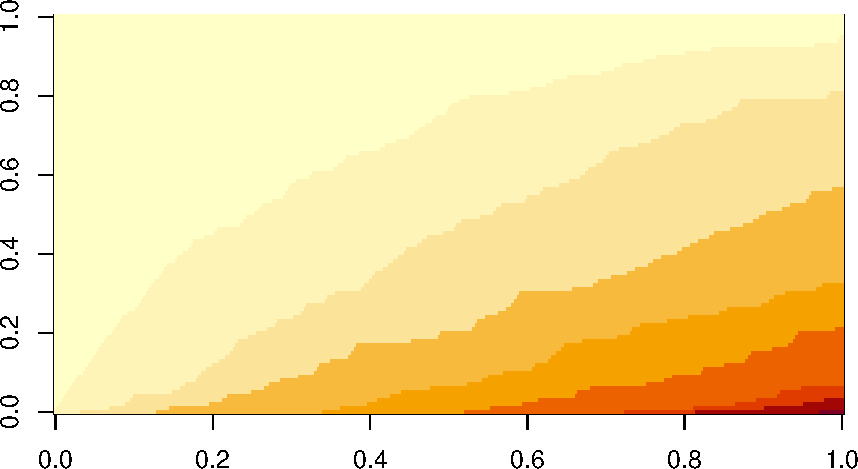
\includegraphics{examples_files/figure-latex/unnamed-chunk-6-1.pdf}

\begin{Shaded}
\begin{Highlighting}[]
\NormalTok{nb\_time }\OtherTok{\textless{}{-}} \FunctionTok{apply}\NormalTok{(res, }\DecValTok{1}\NormalTok{, }\ControlFlowTok{function}\NormalTok{(x) }\FunctionTok{sum}\NormalTok{(x }\SpecialCharTok{\textgreater{}} \DecValTok{0}\NormalTok{))}

\NormalTok{curve }\OtherTok{\textless{}{-}}\NormalTok{ nbCoupons}\SpecialCharTok{*}\NormalTok{(}\DecValTok{1}\SpecialCharTok{{-}}\NormalTok{ (}\DecValTok{1{-}1}\SpecialCharTok{/}\NormalTok{nbCoupons)}\SpecialCharTok{\^{}}\NormalTok{(}\DecValTok{1}\SpecialCharTok{:}\NormalTok{myN))}
\NormalTok{ylimit }\OtherTok{\textless{}{-}} \FunctionTok{max}\NormalTok{(}\FunctionTok{c}\NormalTok{(nb\_time, curve))}
\FunctionTok{plot}\NormalTok{(curve, }\AttributeTok{type =} \StringTok{\textquotesingle{}l\textquotesingle{}}\NormalTok{, }\AttributeTok{ylim =} \FunctionTok{c}\NormalTok{(}\DecValTok{0}\NormalTok{,ylimit), }\AttributeTok{ylab =} \StringTok{""}\NormalTok{)}
\FunctionTok{par}\NormalTok{(}\AttributeTok{new =} \ConstantTok{TRUE}\NormalTok{)}
\FunctionTok{plot}\NormalTok{(nb\_time, }\AttributeTok{type =} \StringTok{\textquotesingle{}l\textquotesingle{}}\NormalTok{, }\AttributeTok{col =} \DecValTok{2}\NormalTok{, }\AttributeTok{ylim =} \FunctionTok{c}\NormalTok{(}\DecValTok{0}\NormalTok{,ylimit), }\AttributeTok{ylab =} \StringTok{"counts"}\NormalTok{)}
\end{Highlighting}
\end{Shaded}

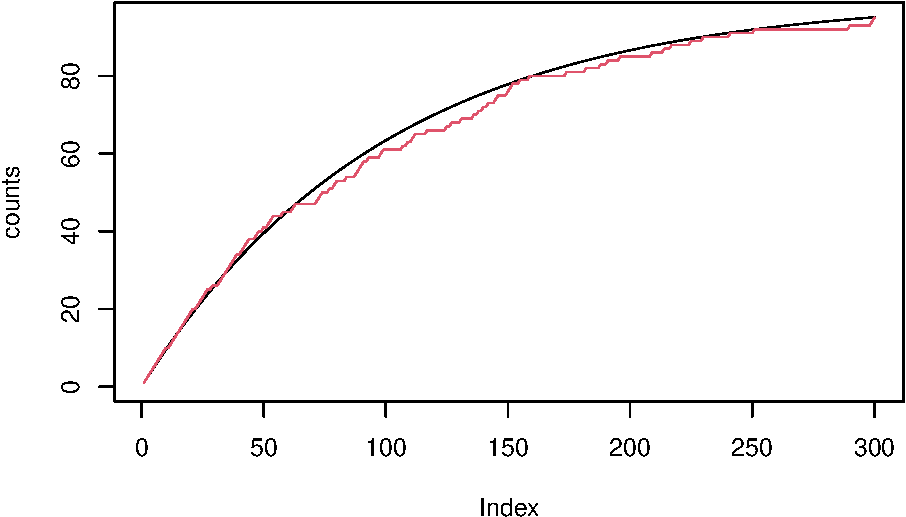
\includegraphics{examples_files/figure-latex/unnamed-chunk-6-2.pdf}

Study of the quality of our estimator

\begin{Shaded}
\begin{Highlighting}[]
\NormalTok{res }\OtherTok{\textless{}{-}} \FunctionTok{replicate}\NormalTok{(}\DecValTok{1000}\NormalTok{, }\FunctionTok{estimatorExpectation}\NormalTok{(}\AttributeTok{nbCoupons =} \DecValTok{200}\NormalTok{,}\AttributeTok{N =} \DecValTok{300}\NormalTok{))}
\FunctionTok{mean}\NormalTok{(}\FunctionTok{unlist}\NormalTok{(res[}\DecValTok{1}\NormalTok{,]))}
\end{Highlighting}
\end{Shaded}

\begin{verbatim}
## [1] 200.617
\end{verbatim}

\begin{Shaded}
\begin{Highlighting}[]
\FunctionTok{sd}\NormalTok{(}\FunctionTok{unlist}\NormalTok{(res[}\DecValTok{1}\NormalTok{,]))}
\end{Highlighting}
\end{Shaded}

\begin{verbatim}
## [1] 12.53728
\end{verbatim}

\begin{Shaded}
\begin{Highlighting}[]
\FunctionTok{mean}\NormalTok{(}\FunctionTok{unlist}\NormalTok{(res[}\DecValTok{2}\NormalTok{,]))}
\end{Highlighting}
\end{Shaded}

\begin{verbatim}
## [1] 155.495
\end{verbatim}

\begin{Shaded}
\begin{Highlighting}[]
\FunctionTok{sd}\NormalTok{(}\FunctionTok{unlist}\NormalTok{(res[}\DecValTok{2}\NormalTok{,]))}
\end{Highlighting}
\end{Shaded}

\begin{verbatim}
## [1] 4.520886
\end{verbatim}

\begin{Shaded}
\begin{Highlighting}[]
\FunctionTok{hist}\NormalTok{(}\FunctionTok{unlist}\NormalTok{(res[}\DecValTok{1}\NormalTok{,]), }\AttributeTok{breaks =} \DecValTok{100}\NormalTok{)}
\end{Highlighting}
\end{Shaded}

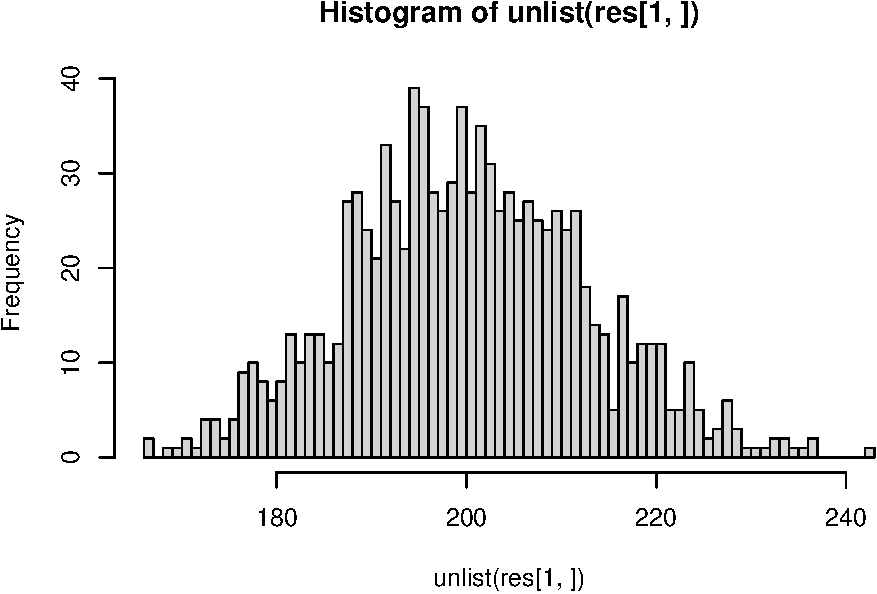
\includegraphics{examples_files/figure-latex/unnamed-chunk-7-1.pdf}

\end{document}
